%%%%%%%%%%%%%%%%%%%%%%%%%%%%%%%%%%%%%%%%%
% Masters/Doctoral Thesis 
% LaTeX Template
% Version 1.43 (17/5/14)
%
% This template has been downloaded from:
% http://www.LaTeXTemplates.com
%
% Original authors:
% Steven Gunn 
% http://users.ecs.soton.ac.uk/srg/softwaretools/document/templates/
% and
% Sunil Patel
% http://www.sunilpatel.co.uk/thesis-template/
%
% License:
% CC BY-NC-SA 3.0 (http://creativecommons.org/licenses/by-nc-sa/3.0/)
%
% Note:
% Make sure to edit document variables in the Thesis.cls file
%
%%%%%%%%%%%%%%%%%%%%%%%%%%%%%%%%%%%%%%%%%

%----------------------------------------------------------------------------------------
%	PACKAGES AND OTHER DOCUMENT CONFIGURATIONS
%----------------------------------------------------------------------------------------

\documentclass[11pt, oneside]{Thesis} % The default font size and one-sided printing (no margin offsets)

\graphicspath{{Pictures/}} % Specifies the directory where pictures are stored

\usepackage[square, numbers, comma, sort&compress]{natbib} % Use the natbib reference package - read up on this to edit the reference style; if you want text (e.g. Smith et al., 2012) for the in-text references (instead of numbers), remove 'numbers' 
\hypersetup{urlcolor=blue, colorlinks=true} % Colors hyperlinks in blue - change to black if annoying
\title{\ttitle} % Defines the thesis title - don't touch this

\begin{document}

\frontmatter % Use roman page numbering style (i, ii, iii, iv...) for the pre-content pages

\setstretch{1.3} % Line spacing of 1.3

% Define the page headers using the FancyHdr package and set up for one-sided printing
\fancyhead{} % Clears all page headers and footers
\rhead{\thepage} % Sets the right side header to show the page number
\lhead{} % Clears the left side page header

\pagestyle{fancy} % Finally, use the "fancy" page style to implement the FancyHdr headers

\newcommand{\HRule}{\rule{\linewidth}{0.5mm}} % New command to make the lines in the title page

% PDF meta-data
\hypersetup{pdftitle={\ttitle}}
\hypersetup{pdfsubject=\subjectname}
\hypersetup{pdfauthor=\authornames}
\hypersetup{pdfkeywords=\keywordnames}

%----------------------------------------------------------------------------------------
%	TITLE PAGE
%----------------------------------------------------------------------------------------

\begin{titlepage}
\begin{center}

\textsc{\LARGE \univname}\\[1.5cm] % University name
\textsc{\Large Doctoral Thesis}\\[0.5cm] % Thesis type

\HRule \\[0.4cm] % Horizontal line
{\huge \bfseries \ttitle}\\[0.4cm] % Thesis title
\HRule \\[1.5cm] % Horizontal line
 
\begin{minipage}{0.4\textwidth}
\begin{flushleft} \large
\emph{Author:}\\
\href{http://www.johnsmith.com}{\authornames} % Author name - remove the \href bracket to remove the link
\end{flushleft}
\end{minipage}
\begin{minipage}{0.4\textwidth}
\begin{flushright} \large
\emph{Supervisor:} \\
\href{http://www.jamessmith.com}{\supname} % Supervisor name - remove the \href bracket to remove the link  
\end{flushright}
\end{minipage}\\[3cm]
 
\large \textit{A thesis submitted in fulfilment of the requirements\\ for the degree of \degreename}\\[0.3cm] % University requirement text
\textit{in the}\\[0.4cm]
\groupname\\\deptname\\[2cm] % Research group name and department name
 
{\large \today}\\[4cm] % Date
%\includegraphics{Logo} % University/department logo - uncomment to place it
 
\vfill
\end{center}

\end{titlepage}

%----------------------------------------------------------------------------------------
%	DECLARATION PAGE
%	Your institution may give you a different text to place here
%----------------------------------------------------------------------------------------

\Declaration{

\addtocontents{toc}{\vspace{1em}} % Add a gap in the Contents, for aesthetics

I, \authornames, declare that this thesis titled, '\ttitle' and the work presented in it are my own. I confirm that:

\begin{itemize} 
\item[\tiny{$\blacksquare$}] This work was done wholly or mainly while in candidature for a research degree at this University.
\item[\tiny{$\blacksquare$}] Where any part of this thesis has previously been submitted for a degree or any other qualification at this University or any other institution, this has been clearly stated.
\item[\tiny{$\blacksquare$}] Where I have consulted the published work of others, this is always clearly attributed.
\item[\tiny{$\blacksquare$}] Where I have quoted from the work of others, the source is always given. With the exception of such quotations, this thesis is entirely my own work.
\item[\tiny{$\blacksquare$}] I have acknowledged all main sources of help.
\item[\tiny{$\blacksquare$}] Where the thesis is based on work done by myself jointly with others, I have made clear exactly what was done by others and what I have contributed myself.\\
\end{itemize}
 
Signed:\\
\rule[1em]{25em}{0.5pt} % This prints a line for the signature
 
Date:\\
\rule[1em]{25em}{0.5pt} % This prints a line to write the date
}

\clearpage % Start a new page

%----------------------------------------------------------------------------------------
%	QUOTATION PAGE
%----------------------------------------------------------------------------------------

\pagestyle{empty} % No headers or footers for the following pages

\null\vfill % Add some space to move the quote down the page a bit

\textit{``Thanks to my solid academic training, today I can write hundreds of words on virtually any topic without possessing a shred of information, which is how I got a good job in journalism."}

\begin{flushright}
Dave Barry
\end{flushright}

\vfill\vfill\vfill\vfill\vfill\vfill\null % Add some space at the bottom to position the quote just right

\clearpage % Start a new page

%----------------------------------------------------------------------------------------
%	ABSTRACT PAGE
%----------------------------------------------------------------------------------------

\addtotoc{Abstract} % Add the "Abstract" page entry to the Contents

\abstract{\addtocontents{toc}{\vspace{1em}} % Add a gap in the Contents, for aesthetics

The Thesis Abstract is written here (and usually kept to just this page). The page is kept centered vertically so can expand into the blank space above the title too\ldots
}

\clearpage % Start a new page

%----------------------------------------------------------------------------------------
%	ACKNOWLEDGEMENTS
%----------------------------------------------------------------------------------------

\setstretch{1.3} % Reset the line-spacing to 1.3 for body text (if it has changed)

\acknowledgements{\addtocontents{toc}{\vspace{1em}} % Add a gap in the Contents, for aesthetics

The acknowledgements and the people to thank go here, don't forget to include your project advisor\ldots
}
\clearpage % Start a new page

%----------------------------------------------------------------------------------------
%	LIST OF CONTENTS/FIGURES/TABLES PAGES
%----------------------------------------------------------------------------------------

\pagestyle{fancy} % The page style headers have been "empty" all this time, now use the "fancy" headers as defined before to bring them back

\lhead{\emph{Contents}} % Set the left side page header to "Contents"
\tableofcontents % Write out the Table of Contents

\lhead{\emph{List of Figures}} % Set the left side page header to "List of Figures"
\listoffigures % Write out the List of Figures

\lhead{\emph{List of Tables}} % Set the left side page header to "List of Tables"
\listoftables % Write out the List of Tables

%----------------------------------------------------------------------------------------
%	ABBREVIATIONS
%----------------------------------------------------------------------------------------

\clearpage % Start a new page

\setstretch{1.5} % Set the line spacing to 1.5, this makes the following tables easier to read

\lhead{\emph{Abbreviations}} % Set the left side page header to "Abbreviations"
\listofsymbols{ll} % Include a list of Abbreviations (a table of two columns)
{
\textbf{LAH} & \textbf{L}ist \textbf{A}bbreviations \textbf{H}ere \\
%\textbf{Acronym} & \textbf{W}hat (it) \textbf{S}tands \textbf{F}or \\
}

%----------------------------------------------------------------------------------------
%	PHYSICAL CONSTANTS/OTHER DEFINITIONS
%----------------------------------------------------------------------------------------

\clearpage % Start a new page

\lhead{\emph{Physical Constants}} % Set the left side page header to "Physical Constants"

\listofconstants{lrcl} % Include a list of Physical Constants (a four column table)
{
Speed of Light & $c$ & $=$ & $2.997\ 924\ 58\times10^{8}\ \mbox{ms}^{-\mbox{s}}$ (exact)\\
% Constant Name & Symbol & = & Constant Value (with units) \\
}

%----------------------------------------------------------------------------------------
%	SYMBOLS
%----------------------------------------------------------------------------------------

\clearpage % Start a new page

\lhead{\emph{Symbols}} % Set the left side page header to "Symbols"

\listofnomenclature{lll} % Include a list of Symbols (a three column table)
{
$a$ & distance & m \\
$P$ & power & W (Js$^{-1}$) \\
% Symbol & Name & Unit \\

& & \\ % Gap to separate the Roman symbols from the Greek

$\omega$ & angular frequency & rads$^{-1}$ \\
% Symbol & Name & Unit \\
}

%----------------------------------------------------------------------------------------
%	DEDICATION
%----------------------------------------------------------------------------------------

\setstretch{1.3} % Return the line spacing back to 1.3

\pagestyle{empty} % Page style needs to be empty for this page

\dedicatory{For/Dedicated to/To my\ldots} % Dedication text

\addtocontents{toc}{\vspace{2em}} % Add a gap in the Contents, for aesthetics

%----------------------------------------------------------------------------------------
%	THESIS CONTENT - CHAPTERS
%----------------------------------------------------------------------------------------

\mainmatter % Begin numeric (1,2,3...) page numbering

\pagestyle{fancy} % Return the page headers back to the "fancy" style

% Include the chapters of the thesis as separate files from the Chapters folder
% Uncomment the lines as you write the chapters

% Chapter 1

\chapter{Chapter Title Here} % Main chapter title

\label{Chapter1} % For referencing the chapter elsewhere, use \ref{Chapter1} 

\lhead{Chapter 1. \emph{Chapter Title Here}} % This is for the header on each page - perhaps a shortened title

%----------------------------------------------------------------------------------------

\section{Welcome and Thank You}
Welcome to this \LaTeX{} Thesis Template, a beautiful and easy to use template for writing a thesis using the \LaTeX{} typesetting system.

If you are writing a thesis (or will be in the future) and its subject is technical or mathematical (though it doesn't have to be), then creating it in \LaTeX{} is highly recommended as a way to make sure you can just get down to the essential writing without having to worry over formatting or wasting time arguing with your word processor.

\LaTeX{} is easily able to professionally typeset documents that run to hundreds or thousands of pages long. With simple mark-up commands, it automatically sets out the table of contents, margins, page headers and footers and keeps the formatting consistent and beautiful. One of its main strengths is the way it can easily typeset mathematics, even \emph{heavy} mathematics. Even if those equations are the most horribly twisted and most difficult mathematical problems that can only be solved on a super-computer, you can at least count on \LaTeX{} to make them look stunning.

%----------------------------------------------------------------------------------------

\section{Learning \LaTeX{}}

\LaTeX{} is not a WYSIWYG (What You See is What You Get) program, unlike word processors such as Microsoft Word or Apple's Pages. Instead, a document written for \LaTeX{} is actually a simple, plain text file that contains \emph{no formatting}. You tell \LaTeX{} how you want the formatting in the finished document by writing in simple commands amongst the text, for example, if I want to use \textit{italic text for emphasis}, I write the `$\backslash$\texttt{textit}\{\}' command and put the text I want in italics in between the curly braces. This means that \LaTeX{} is a ``mark-up'' language, very much like HTML.

\subsection{A (not so short) Introduction to \LaTeX{}}

If you are new to \LaTeX{}, there is a very good eBook -- freely available online as a PDF file -- called, ``The Not So Short Introduction to \LaTeX{}''. The book's title is typically shortened to just ``lshort''. You can download the latest version (as it is occasionally updated) from here:\\
\href{http://www.ctan.org/tex-archive/info/lshort/english/lshort.pdf}{\texttt{http://www.ctan.org/tex-archive/info/lshort/english/lshort.pdf}}

It is also available in several other languages. Find yours from the list on this page:\\
\href{http://www.ctan.org/tex-archive/info/lshort/}{\texttt{http://www.ctan.org/tex-archive/info/lshort/}}

It is recommended to take a little time out to learn how to use \LaTeX{} by creating several, small `test' documents. Making the effort now means you're not stuck learning the system when what you \emph{really} need to be doing is writing your thesis.

\subsection{A Short Math Guide for \LaTeX{}}

If you are writing a technical or mathematical thesis, then you may want to read the document by the AMS (American Mathematical Society) called, ``A Short Math Guide for \LaTeX{}''. It can be found online here:\\
\href{http://www.ams.org/tex/amslatex.html}{\texttt{http://www.ams.org/tex/amslatex.html}}\\
under the ``Additional Documentation'' section towards the bottom of the page.

\subsection{Common \LaTeX{} Math Symbols}
There are a multitude of mathematical symbols available for \LaTeX{} and it would take a great effort to learn the commands for them all. The most common ones you are likely to use are shown on this page:\\
\href{http://www.sunilpatel.co.uk/latexsymbols.html}{\texttt{http://www.sunilpatel.co.uk/latexsymbols.html}}

You can use this page as a reference or crib sheet, the symbols are rendered as large, high quality images so you can quickly find the \LaTeX{} command for the symbol you need.

\subsection{\LaTeX{} on a Mac}
 
The \LaTeX{} package is available for many systems including Windows, Linux and Mac OS X. The package for OS X is called MacTeX and it contains all the applications you need -- bundled together and pre-customised -- for a fully working \LaTeX{} environment and workflow.
 
MacTeX includes a dedicated \LaTeX{} IDE (Integrated Development Environment) called ``TeXShop'' for writing your `\texttt{.tex}' files and ``BibDesk'': a program to manage your references and create your bibliography section just as easily as managing songs and creating playlists in iTunes.

%----------------------------------------------------------------------------------------

\section{Getting Started with this Template}

If you are familiar with \LaTeX{}, then you can familiarise yourself with the contents of the Zip file and the directory structure and then place your own information into the `\texttt{Thesis.cls}' file. Section \ref{FillingFile} on page \pageref{FillingFile} tells you how to do this. Make sure you read section \ref{ThesisConventions} about thesis conventions to get the most out of this template and then get started with the `\texttt{Thesis.tex}' file straightaway.

If you are new to \LaTeX{} it is recommended that you carry on reading through the rest of the information in this document.

\subsection{About this Template}

This \LaTeX{} Thesis Template is originally based and created around a \LaTeX{} style file created by Steve R.\ Gunn from the University of Southampton (UK), department of Electronics and Computer Science. You can find his original thesis style file at his site, here:\\
\href{http://www.ecs.soton.ac.uk/~srg/softwaretools/document/templates/}{\texttt{http://www.ecs.soton.ac.uk/$\sim$srg/softwaretools/document/templates/}}

My thesis originally used the `\texttt{ecsthesis.cls}' from his list of styles. However, I knew \LaTeX{} could still format better. To get the look I wanted, I modified his style and also created a skeleton framework and folder structure to place the thesis files in.

This Thesis Template consists of that modified style, the framework and the folder structure. All the work that has gone into the preparation and groundwork means that all you have to bother about is the writing.

Before you begin using this template you should ensure that its style complies with the thesis style guidelines imposed by your institution. In most cases this template style and layout will be suitable. If it is not, it may only require a small change to bring the template in line with your institution's recommendations.

%----------------------------------------------------------------------------------------

\section{What this Template Includes}

\subsection{Folders}

This template comes as a single Zip file that expands out to many files and folders. The folder names are mostly self-explanatory:

\textbf{Appendices} -- this is the folder where you put the appendices. Each appendix should go into its own separate `\texttt{.tex}' file. A template is included in the directory.

\textbf{Chapters} -- this is the folder where you put the thesis chapters. A thesis usually has about seven chapters, though there is no hard rule on this. Each chapter should go in its own separate `\texttt{.tex}' file and they usually are split as:
\begin{itemize}
\item Chapter 1: Introduction to the thesis topic
\item Chapter 2: Background information and theory
\item Chapter 3: (Laboratory) experimental setup
\item Chapter 4: Details of experiment 1
\item Chapter 5: Details of experiment 2
\item Chapter 6: Discussion of the experimental results
\item Chapter 7: Conclusion and future directions
\end{itemize}
This chapter layout is specialised for the experimental sciences.

\textbf{Figures} -- this folder contains all figures for the thesis. These are the final images that will go into the thesis document.

\textbf{Primitives} -- this is the folder that contains scraps, particularly because one final image in the `Figures' folder may be made from many separate images and photos, these source images go here. This keeps the intermediate files separate from the final thesis figures.

\subsection{Files}

Included are also several files, most of them are plain text and you can see their contents in a text editor. Luckily, many of them are auxiliary files created by \LaTeX{} or BibTeX and which you don't need to bother about:

\textbf{Bibliography.bib} -- this is an important file that contains all the bibliographic information and references that you will be citing in the thesis for use with BibTeX. You can write it manually, but there are reference manager programs available that will create and manage it for you. Bibliographies in \LaTeX{} are a large subject and you may need to read about BibTeX before starting with this.

\textbf{Thesis.cls} -- this is an important file. It is the style file that tells \LaTeX{} how to format the thesis. You will also need to open this file in a text editor and fill in your own information (such as name, department, institution). Luckily, this is not too difficult and is explained in section \ref{FillingFile} on page \pageref{FillingFile}.

\textbf{Thesis.pdf} -- this is your beautifully typeset thesis (in the PDF file format) created by \LaTeX{}.

\textbf{Thesis.tex} -- this is an important file. This is the file that you tell \LaTeX{} to compile to produce your thesis as a PDF file. It contains the framework and constructs that tell \LaTeX{} how to layout the thesis. It is heavily commented so you can read exactly what each line of code does and why it is there. After you put your own information into the `\texttt{Thesis.cls}' file, go to this file and begin filling it in -- you have now started your thesis!

\textbf{vector.sty} -- this is a \LaTeX{} package, it tells \LaTeX{} how to typeset mathematical vectors. Using this package is very easy and you can read the documentation on the site (you just need to look at the `\texttt{vector.pdf}' file):\\
\href{http://www.ctan.org/tex-archive/macros/latex/contrib/vector/}{\texttt{http://www.ctan.org/tex-archive/macros/latex/contrib/vector/}}

\textbf{lstpatch.sty} -- this is a \LaTeX{} package required by this LaTeX template and is included as not all \TeX{} distributions have it installed by default. You do not need to modify this file.

Files that are \emph{not} included, but are created by \LaTeX{} as auxiliary files include:

\textbf{Thesis.aux} -- this is an auxiliary file generated by \LaTeX{}, if it is deleted \LaTeX{} simply regenerates it when you run the main `\texttt{.tex}' file.

\textbf{Thesis.bbl} -- this is an auxiliary file generated by BibTeX, if it is deleted, BibTeX simply regenerates it when you run the main tex file. Whereas the `\texttt{.bib}' file contains all the references you have, this `\texttt{.bbl}' file contains the references you have actually cited in the thesis and is used to build the bibliography section of the thesis.

\textbf{Thesis.blg} -- this is an auxiliary file generated by BibTeX, if it is deleted BibTeX simply regenerates it when you run the main `\texttt{.tex}' file.

\textbf{Thesis.lof} -- this is an auxiliary file generated by \LaTeX{}, if it is deleted \LaTeX{} simply regenerates it when you run the main `\texttt{.tex}' file. It tells \LaTeX{} how to build the `List of Figures' section.

\textbf{Thesis.log} -- this is an auxiliary file generated by \LaTeX{}, if it is deleted \LaTeX{} simply regenerates it when you run the main `\texttt{.tex}' file. It contains messages from \LaTeX{}, if you receive errors and warnings from \LaTeX{}, they will be in this `\texttt{.log}' file.

\textbf{Thesis.lot} -- this is an auxiliary file generated by \LaTeX{}, if it is deleted \LaTeX{} simply regenerates it when you run the main `\texttt{.tex}' file. It tells \LaTeX{} how to build the `List of Tables' section.

\textbf{Thesis.out} -- this is an auxiliary file generated by \LaTeX{}, if it is deleted \LaTeX{} simply regenerates it when you run the main `\texttt{.tex}' file.


So from this long list, only the files with the `\texttt{.sty}', `\texttt{.bib}', `\texttt{.cls}' and `\texttt{.tex}' extensions are the most important ones. The other auxiliary files can be ignored or deleted as \LaTeX{} and BibTeX will regenerate them.

%----------------------------------------------------------------------------------------

\section{Filling in the `\texttt{Thesis.cls}' File}\label{FillingFile}

You will need to personalise the thesis template and make it your own by filling in your own information. This is done by editing the `\texttt{Thesis.cls}' file in a text editor.

Open the file and scroll down, past all the `$\backslash$\texttt{newcommand}\ldots' items until you see the entries for `\texttt{University Name}', `\texttt{Department Name}', etc\ldots.

Fill out the information about your group and institution and ensure you keep to block capitals where it asks you to. You can also insert web links, if you do, make sure you use the full URL, including the `\texttt{http://}' for this.

The last item you should need to fill in is the Faculty Name (in block capitals). When you have done this, save the file and recompile `\texttt{Thesis.tex}'. All the information you filled in should now be in the PDF, complete with web links. You can now begin your thesis proper!

%----------------------------------------------------------------------------------------

\section{The `\texttt{Thesis.tex}' File Explained}

The \texttt{Thesis.tex} file contains the structure of the thesis. There are plenty of written comments that explain what pages, sections and formatting the \LaTeX{} code is creating. Initially there seems to be a lot of \LaTeX{} code, but this is all formatting, and it has all been taken care of so you don't have to do it.

Begin by checking that your information on the title page is correct. For the thesis declaration, your institution may insist on something different than the text given. If this is the case, just replace what you see with what is required.

Then comes a page which contains a funny quote. You can put your own, or quote your favourite scientist, author, person, etc\ldots Make sure to put the name of the person who you took the quote from.

Next comes the acknowledgements. On this page, write about all the people who you wish to thank (not forgetting parents, partners and your advisor/supervisor).

The contents pages, list of figures and tables are all taken care of for you and do not need to be manually created or edited. The next set of pages are optional and can be deleted since they are for a more technical thesis: insert a list of abbreviations you have used in the thesis, then a list of the physical constants and numbers you refer to and finally, a list of mathematical symbols used in any formulae. Making the effort to fill these tables means the reader has a one-stop place to refer to instead of searching the internet and references to try and find out what you meant by certain abbreviations or symbols.

The list of symbols is split into the Roman and Greek alphabets. Whereas the abbreviations and symbols ought to be listed in alphabetical order (and this is \emph{not} done automatically for you) the list of physical constants should be grouped into similar themes.

The next page contains a one line dedication. Who will you dedicate your thesis to?

Finally, there is the section where the chapters are included. Uncomment the lines (delete the `\texttt{\%}' character) as you write the chapters. Each chapter should be written in its own file and put into the `Chapters' folder and named `\texttt{Chapter1}', `\texttt{Chapter2}, etc\ldots Similarly for the appendices, uncomment the lines as you need them. Each appendix should go into its own file and placed in the `Appendices' folder.

After the preamble, chapters and appendices finally comes the bibliography. The bibliography style (called `\texttt{unsrtnat}') is used for the bibliography and is a fully featured style that will even include links to where the referenced paper can be found online. Do not under estimate how grateful you reader will be to find that a reference to a paper is just a click away. Of course, this relies on you putting the URL information into the BibTeX file in the first place.

%----------------------------------------------------------------------------------------

\section{Thesis Features and Conventions}\label{ThesisConventions}

To get the best out of this template, there are a few conventions that you may want to follow.

One of the most important (and most difficult) things to keep track of in such a long document as a thesis is consistency. Using certain conventions and ways of doing things (such as using a Todo list) makes the job easier. Of course, all of these are optional and you can adopt your own method.

\subsection{Printing Format}

This thesis template is designed for single sided printing as most theses are printed and bound this way. This means that the left margin is always wider than the right (for binding). Four out of five people will now judge the margins by eye and think, ``I never 
noticed that before.''.

The headers for the pages contain the page number on the right side (so it is easy to flick through to the page you want) and the chapter name on the left side.

The text is set to 11 point and a line spacing of 1.3. Generally, it is much more readable to have a smaller text size and wider gap between the lines than it is to have a larger text size and smaller gap. Again, you can tune the text size and spacing should you want or need to. The text size can be set in the options for the `$\backslash$\texttt{documentclass}' command at the top of the `\texttt{Thesis.tex}' file and the spacing can be changed by setting a different value in the `$\backslash$\texttt{setstretch}' commands (scattered throughout the `\texttt{Thesis.tex}' file).

\subsection{Using US Letter Paper}

The paper size used in the template is A4, which is a common -- if not standard -- size in Europe. If you are using this thesis template elsewhere and particularly in the United States, then you may have to change the A4 paper size to the US Letter size. Unfortunately, this is not as simple as replacing instances of `\texttt{a4paper}' with `\texttt{letterpaper}'.

This is because the final PDF file is created directly from the \LaTeX{} source using a program called `\texttt{pdfTeX}' and in certain conditions, paper size commands are ignored and all documents are created with the paper size set to the size stated in the configuration file for pdfTeX (called `\texttt{pdftex.cfg}').

What needs to be done is to change the paper size in the configuration file for \texttt{pdfTeX} to reflect the letter size. There is an excellent tutorial on how to do this here: \\
\href{http://www.physics.wm.edu/~norman/latexhints/pdf_papersize.html}{\texttt{http://www.physics.wm.edu/$\sim$norman/latexhints/pdf\_papersize.html}}

It may be sufficient just to replace the dimensions of the A4 paper size with the US Letter size in the \texttt{pdftex.cfg} file. Due to the differences in the paper size, the resulting margins may be different to what you like or require (as it is common for Institutions to dictate certain margin sizes). If this is the case, then the margin sizes can be tweaked by opening up the \texttt{Thesis.cls} file and searching for the line beginning with, `$\backslash$\texttt{setmarginsrb}' (not very far down from the top), there you will see the margins specified. Simply change those values to what you need (or what looks good) and save. Now your document should be set up for US Letter paper size with suitable margins.

\subsection{References}

The `\texttt{natbib}' package is used to format the bibliography and inserts references such as this one \citep{Reference3}. The options used in the `\texttt{Thesis.tex}' file mean that the references are listed in numerical order as they appear in the text. Multiple references are rearranged in numerical order (e.g. \citep{Reference2, Reference1}) and multiple, sequential references become reformatted to a reference range (e.g. \citep{Reference2, Reference1, Reference3}). This is done automatically for you. To see how you use references, have a look at the `\texttt{Chapter1.tex}' source file. Many reference managers allow you to simply drag the reference into the document as you type.

Scientific references should come \emph{before} the punctuation mark if there is one (such as a comma or period). The same goes for footnotes\footnote{Such as this footnote, here down at the bottom of the page.}. You can change this but the most important thing is to keep the convention consistent throughout the thesis. Footnotes themselves should be full, descriptive sentences (beginning with a capital letter and ending with a full stop).

To see how \LaTeX{} typesets the bibliography, have a look at the very end of this document (or just click on the reference number links).

\subsection{Figures}

There will hopefully be many figures in your thesis (that should be placed in the `Figures' folder). The way to insert figures into your thesis is to use a code template like this:
\begin{verbatim}
\begin{figure}[htbp]
  \centering
    
\includegraphics{Figures/Electron.pdf}
    \rule{35em}{0.5pt}
  \caption[An Electron]{An electron (artist's impression).}
  \label{fig:Electron}
\end{figure}
\end{verbatim}
Also look in the source file. Putting this code into the source file produces the picture of the electron that you can see in the figure below.

\begin{figure}[htbp]
	\centering
		
\includegraphics{Figures/Electron.pdf}
		\rule{35em}{0.5pt}
	\caption[An Electron]{An electron (artist's impression).}
	\label{fig:Electron}
\end{figure}

Sometimes figures don't always appear where you write them in the source. The placement depends on how much space there is on the page for the figure. Sometimes there is not enough room to fit a figure directly where it should go (in relation to the text) and so \LaTeX{} puts it at the top of the next page. Positioning figures is the job of \LaTeX{} and so you should only worry about making them look good!

Figures usually should have labels just in case you need to refer to them (such as in Figure \ref{fig:Electron}). The `$\backslash$\texttt{caption}' command contains two parts, the first part, inside the square brackets is the title that will appear in the `List of Figures', and so should be short. The second part in the curly brackets should contain the longer and more descriptive caption text.

The `$\backslash$\texttt{rule}' command is optional and simply puts an aesthetic horizontal line below the image. If you do this for one image, do it for all of them.

The \LaTeX{} Thesis Template is able to use figures that are either in the PDF or JPEG file format.

\subsection{Typesetting mathematics}

If your thesis is going to contain heavy mathematical content, be sure that \LaTeX{} will make it look beautiful, even though it won't be able to solve the equations for you.

The ``Not So Short Introduction to \LaTeX{}'' (available \href{http://www.ctan.org/tex-archive/info/lshort/english/lshort.pdf}{here}) should tell you everything you need to know for most cases of typesetting mathematics. If you need more information, a much more thorough mathematical guide is available from the AMS called, ``A Short Math Guide to \LaTeX{}'' and can be downloaded from:\\
\href{ftp://ftp.ams.org/pub/tex/doc/amsmath/short-math-guide.pdf}{\texttt{ftp://ftp.ams.org/pub/tex/doc/amsmath/short-math-guide.pdf}}

There are many different \LaTeX{} symbols to remember, luckily you can find the most common symbols \href{http://www.sunilpatel.co.uk/latexsymbols.html}{here}. You can use the web page as a quick reference or crib sheet and because the symbols are grouped and rendered as high quality images (each with a downloadable PDF), finding the symbol you need is quick and easy.

You can write an equation, which is automatically given an equation number by \LaTeX{} like this:
\begin{verbatim}
\begin{equation}
E = mc^{2}
  \label{eqn:Einstein}
\end{equation}
\end{verbatim}

This will produce Einstein's famous energy-matter equivalence equation:
\begin{equation}
E = mc^{2}
\label{eqn:Einstein}
\end{equation}

All equations you write (which are not in the middle of paragraph text) are automatically given equation numbers by \LaTeX{}. If you don't want a particular equation numbered, just put the command, `$\backslash$\texttt{nonumber}' immediately after the equation.

%----------------------------------------------------------------------------------------

\section{Sectioning and Subsectioning}

You should break your thesis up into nice, bite-sized sections and subsections. \LaTeX{} automatically builds a table of Contents by looking at all the `$\backslash$\texttt{chapter}$\{\}$', `$\backslash$\texttt{section}$\{\}$' and `$\backslash$\texttt{subsection}$\{\}$' commands you write in the source.

The table of Contents should only list the sections to three (3) levels. A `$\backslash$\texttt{chapter}$\{\}$' is level one (1). A `$\backslash$\texttt{section}$\{\}$' is level two (2) and so a `$\backslash$\texttt{subsection}$\{\}$' is level three (3). In your thesis it is likely that you will even use a `$\backslash$\texttt{subsubsection}$\{\}$', which is level four (4). Adding all these will create an unnecessarily cluttered table of Contents and so you should use the `$\backslash$\texttt{subsubsection$^{*}\{\}$}' command instead (note the asterisk). The asterisk ($^{*}$) tells \LaTeX{} to omit listing the subsubsection in the Contents, keeping it clean and tidy.

%----------------------------------------------------------------------------------------

\section{In Closing}

You have reached the end of this mini-guide. You can now rename or overwrite this pdf file and begin writing your own `\texttt{Chapter1.tex}' and the rest of your thesis. The easy work of setting up the structure and framework has been taken care of for you. It's now your job to fill it out!

Good luck and have lots of fun!

\begin{flushright}
Guide written by ---\\
Sunil Patel: \href{http://www.sunilpatel.co.uk}{www.sunilpatel.co.uk}
\end{flushright}

%% Chapter 2

\yyyymmdddate
\renewcommand{\dateseparator}{-}
\newcommand{\tabitem}{~~\llap{\textbullet}~~}

\renewcommand*\ttdefault{txtt}
\newcommand{\ms}[1]{\mbox{\tt #1}\xspace}
\newcommand{\seq}{{\bf s}\xspace}
\newcommand{\strS}{{\mathcal S}\xspace}
\newcommand{\strOff}{\ensuremath{{\mathcal S}_{\text{off}}}\xspace}
\newcommand{\strOn}{\ensuremath{{\mathcal S}_{\text{on}}}\xspace}
\newcommand{\strConst}[1]{\ensuremath{{\mathcal C}_{\text{#1}}}\xspace}
\newcommand{\tree}{{\mathcal T}\xspace}
\newcommand{\treeFor}[1]{\ensuremath{{\mathcal T}_{\text #1}}}
\newcommand{\fnaRetrievalTime}{\formatdate{25}{11}{2014} at \formattime{9}{14}{0}}
\newcommand{\textdown}[2]{\ensuremath{{\text{#1}}_{\text{#2}}}}
\newcommand{\treePos}[2]{\textdown{\ms{#1}}{#2}}
\newcommand{\treeIdx}[3]{\treePos{#1}{#2}\ensuremath{(#3)}}

\newcommand{\rfinder}{\ms{Ribofinder}}
\newcommand{\infernal}{\ms{Infernal}}
\newcommand{\tthp}{\ms{TransTermHP}}
\newcommand{\rshapes}{\ms{RNAshapes}}
\newcommand{\rfold}{\ms{RNAfold}}
\newcommand{\foldalign}{\ms{FoldAlign}}

\chapter{Ribofinder} % Main chapter title

\label{Chapter2} % For referencing the chapter elsewhere, use \ref{Chapter1}

\lhead{Chapter 2. \emph{Ribofinder: A Riboswitch Detection Pipeline}} % This is for the header on each page - perhaps a shortened title

%----------------------------------------------------------------------------------------

% \begin{abstract}
%   Riboswitches are regulatory mRNA elements that modulate gene expression via structural changes induced by the direct sensing of a small-molecule metabolite. Most often found in bacteria, riboswitches regulate diverse pathways including the metabolism and transport of purines, methionine, and thiamin amongst others. The structure of a riboswitch includes an aptamer domain---involved in the direct sensing of the small-molecule---and an expression platform whose structure changes upon the aptamer binding the metabolite. Because of the discriminatory nature of metabolite sensing, groups have had great success in finding representative examples of aptamers across a diverse collection of bacterial species; RFam 12.0 currently contains 26 different families of aptamers involved in different metabolic pathways. Whereas there exists strong sequence and structural similarity within the aptamer of a riboswitch family, the expression platform is highly variable, and thus challenging to capture using traditional SCFG-based approaches. For this reason databases such as RFam only contain the aptamer portion of the riboswitch, and there exists no database providing sequences including expression platforms, necessary for capturing the `on' and `off' conformations of this regulatory element. We have developed a new pipeline---called \rfinder---which can detect putative riboswitches including their expression platforms and likely conformational structures across a wide collection of genomic sequences.
% \end{abstract}

\section{Pipeline} \label{sec:pipeline}

At the time of our retrieval (\fnaRetrievalTime), the RefSeq database hosted by NCBI comprised 5,121 complete bacterial genomes with corresponding genomic annotations. In order to both detect putative full riboswitches across this collection of data as well as filter the candidates down to a number tractable for experimental validation, we developed a novel pipeline which takes a three-tiered approach to candidate selection. Our approach is to \begin{inparaenum}[\itshape a\upshape)]
\item identify a pool of candidate riboswitches across genomic data;
\item perform a coarse-grained filtering of the candidate pool based on structural characteristics; and finally
\item fine-grained curation of the candidates based on a collection of measures and pairwise similarity.
\end{inparaenum}

In the following discussion, we describe the application of \rfinder to identify unannotated G-box purine riboswitches; guanine-sensing cis-regulatory elements which modulate the expression of genes involved in purine biosynthesis.

\subsection{Candidate Selection} \label{sub:candidates}

The RefSeq data we used for analysis contains 5,121 annotated bacterial genomes across 2,732 different organisms, totaling over $9.5 * 10^9$ bases. We used the program \infernal to determine the coordinates of putative aptamer structures within the RefSeq genomes, and \tthp to locate candidate rho-independent transcription terminators.

\subsubsection{Detecting Aptamers with \infernal} \label{ssub:infernal}

\infernal uses a stochastic context-free grammar (SCFG) with a user-provided multiple sequence alignment (MSA) to efficiently scan genomic data for RNA homologs, taking into consideration both sequence and structural conservation. Using the purine aptamer MSA from RFam 12.0 (RF00167), \infernal (v1.1.1, default options) detects 1,537 significant hits having E-value $<= 0.01$. Because \infernal leverages the concept of a `local end'---a large insertion or deletion in the alignment at reduced cost---it is possible for the software to return a significant hit whose aligned structure does not have the canonical three-way junction observed in all purine riboswitches. \rfinder prunes these truncated \infernal hits by converting the alignment structure into a parse tree, and only permitting trees of sufficient complexity to contain a multiloop (described further in \ref{sub:shapes}). The pyrimidine residue abutted next to the P1 stem in the J3-1 junction differentiates between guanine and adenine-sensing riboswitches by binding the complimentary purine ligand; for our interest in G-box riboswitches exclusively we require the presence of a cytosine at this residue. In total, using \infernal with these additional filters yields 1,280 G-box aptamers across 555 unique organisms (note: here and elsewhere I define a `unique organism' as having a unique taxonomy ID).

\subsubsection{Detecting Expression Platforms with \tthp} \label{ssub:tthp}

\tthp detects rho-independent terminators in bacterial genomes in a context-sensitive fashion by leveraging the protein annotations available in PTT data. These terminator sequences canonically have a stable hairpin loop structure immediately preceding a run of $5+$ uracil residues, the combination of which causes the ribosomal machinery to stall and dissociate from the transcript. \tthp performs a genomic scan to determine candidate loci with this motif, and returns scored hits. The scoring system considers both structural homology and the genomic contextual information available in the PTT file. Across our collection of bacterial genomes acquired from NCBI RefSeq data, \tthp identified 2,752,469 rho-independent terminators using the default filters.

Due to the spatially-mediated structural regulation of purine riboswitches, whereby ligand interaction with the aptamer domain induces local structural rearrangement in the expression platform, we paired aptamers with corresponding terminators by minimizing the genomic distance, with an upper bound of 200 nucleotides between the end of the aptamer domain and start of the terminator. This approach yields 577 candidate riboswitches, 81 of which have multiple rho-independent terminators within range of a putative aptamer produced by \infernal. For these, we simply pair the closest \tthp hit with the aptamer domain.

\begin{figure}[!ht]
  \centering
    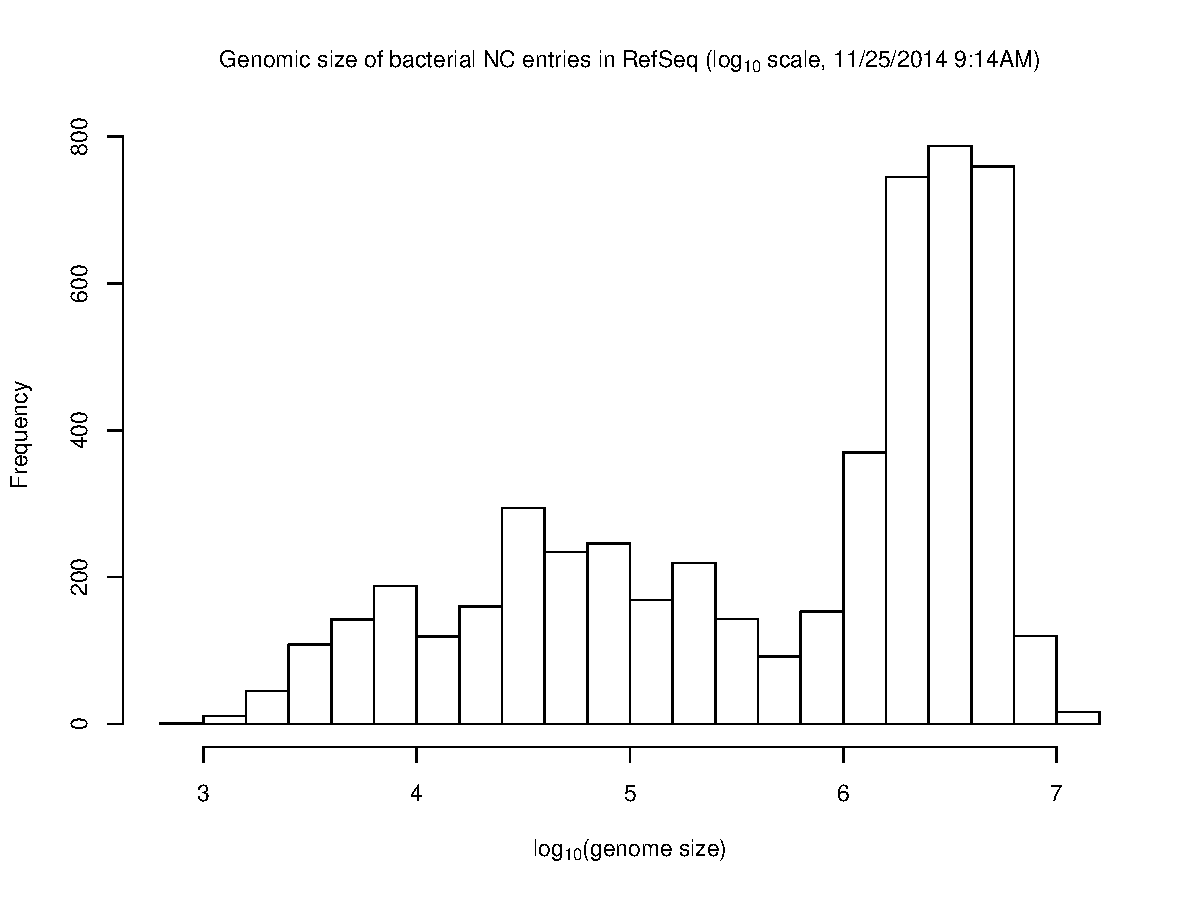
\includegraphics[width=.75\linewidth]{Figures/refseq_genome_sizes.pdf}
  \caption{Histogram displaying the distribution of genome sizes across the RefSeq data analyzed, comprising 5,172 bacterial genomes. Genome size is shown using a $\log_{10}$ scale.}
  \label{fig:genome_sizes}
\end{figure}

\subsection{Notation for Representing Abstract RNA Shapes} \label{sub:shapes}

Given an RNA sequence $\seq = a_1, a_2, \cdots, a_n$, where positions $a_i$ are drawn from the collection of single-letter nucleotide codes, i.e. $\{\text{A},\text{U},\text{G},\text{C}\}$, it is possible to describe a corresponding secondary structure $\strS$ compatible with $\seq$ using the dot-bracket notation. In this notation, each nucleotide $a_i$ has a corresponding state $s_i$, where $s_i$ is denoted as a `.' if unpaired and a `(' [resp. `)'] if the left [resp. right] base in a basepair. Given any two basepairs $(i,j)$ and $(k,l)$ in $\strS$, then $i < k < j \iff i < l < j$; pseudoknots are not permitted in the structure. A secondary structure taking this form is said to have balanced parentheses, and can additionally be represented using a context-free grammar such as:

\begin{equation} \label{eq:str_cfg}
S \rightarrow S\,.\;|\;.\,S\;|\;(S)\;|\;SS\;|\;\epsilon
\end{equation}

The grammar from \eqref{eq:str_cfg} can be used to generate a parse tree $\tree$ for $\strS$. The benefit of working with $\tree$ over $\strS$ is that the parse tree offers an abstract representation of secondary structure shape independent of sequence length, permitting us to classify and eventually constrain a large collection of sequences having variable length which are all expected to have the same abstract tree shape. This is analogous to what the Giegerich lab refers to as their `type 5' structural abstraction using the \rshapes tool. Every node in $\tree$ represents a helix in $\strS$, and internally tracks the indices of both its beginning $(i,j)$ and closing $(k,l)$ basepair. We use a level-order naming convention to refer to helices within the parse tree, whereby a position \treePos{p}{1} references the first child of the root node, \treePos{p}{1,2} references the second child of \textdown{\ms{p}}{1}, and generally \treePos{p}{$i_1,i_2,\cdots,i_n$} refers to the $i_n$\textsuperscript{th} child of \treePos{p}{$i_1,i_2,\cdots,i_{n-1}$}. To reference specific nucleotides in the context of their location relative to a helix, we use the opening and closing basepairs $(i,j)$ and $(k,l)$ as landmarks. Thus, \treeIdx{p}{1}{l} is the index in $\strS$ of the right-hand side closing basepair of \treePos{p}{1}. We use the notation \treePos{t}{$i$} to refer to the subtree of $\tree$ whose root is \treePos{p}{$i$}.

Finally, we introduce the concept of a tree signature. The tree signature for a tree $\tree$ is a list of the node depths when traversed in a depth-first pre-order fashion. To provide a concrete example, consider the following experimentally validated xpt G-box riboswitch from Bacillus subtilis subsp. subtilis str. 168 (NC\_000964.3 2320197-2320054) with corresponding gene-off structure:

\begin{center} \label{}
  \ssmall\tt ACACUCAUAUAAUCGCGUGGAUAUGGCACGCAAGUUUCUACCGGGCACCGUAAAUGUCCGACUAUGGGUGAGCAAUGGAACCGCACGUGUACGGUUUUUUGUGAUAUCAGCAUUGCUUGCUCUUUAUUUGAGCGGGCAAUGCUU
  \ssmall\tt .((((((((.....(((((.......)))))..........((((((.......))))))..)))))))).((((.(((((((........)))))))))))......((((((((((((((.......)))))))))))))).
\end{center}

The \rshapes `type 5' representation for this structure is \ms{[[][]][][]} (note the coalesced left bulge in the hairpin immediately downstream the closing multiloop stem, at helix \treePos{p}{2}) and the tree signature for this parse tree of the structure is \ms{[0, 1, 2, 2, 1, 1]}.

\subsection{Coarse-Grained Filtering} \label{sub:coarse}

We leverage the notion of abstract structural filtering initially to ensure that all \infernal aptamer hits have a tree signature of \ms{[0, 1, 2, 2]}, which represents a three-way junction, and that the binding site for the guanine ligand $\treeIdx{p}{1}{l - 1} = \text{C}$. These filters, in combination with the proximal terminator hairpins produced by \tthp yield the aforementioned 577 candidate guanine riboswitches for which we then try to produce reasonable gene-on and off structures.

\subsubsection{Constrained Folding to Predict Switch Structures} \label{ssub:constfold}

To restrict our search to unannotated G-box riboswitches, and further ensure that we are not re-detecting sequences based off the RFam covariance model provided to \infernal, we constrain our search to those RefSeq organisms not represented in the RFam seed alignment. 503 of the 577 candidates, or 87.18\% represent putative unannotated riboswitches not represented by RF00167.

The gene-off structure \strOff for a G-box riboswitch is the easier of the two to find computationally, since the terminator loop is exceptionally thermodynamically stable. In the gene-on conformation \strOn, the P1 stem of the multiloop partially dissociates and an anti-terminator loop forms between the region immediately 3' of the P1 stem and what was the left-hand side of the terminator loop. This truncated P1 stem, which closes the three-way junction in the aptamer, is exceptionally unstable based on present energy models available for structural folding, and requires special treatment to reconstitute in our final structures.

The software \rfold (v2.1.8) allows for the folding of RNA molecules with `loose' constraints. In this model of constrained folding, the resulting structure produced by the software guarantees not to explicitly invalidate any user-provided constraints, but does not guarantee all constraints will be satisfied in the resulting structure. For each of the candidate guanine riboswitches, having \treeFor{\infernal} and \treeFor{\tthp}, we build the following constraint masks:

\begin{center}
\begin{tabular}{p{0.45\linewidth} | p{0.45\linewidth}}
  G-box gene-off constraint mask & G-box gene-on constraint mask \\
  \hline
  \multicolumn{2}{c}{Prohibit basepairing upstream of \treeIdx{p}{1}{i} and downstream of \treeIdx{p}{2}{l}.} \\
  \multicolumn{2}{c}{Force basepairs and unpaired regions in \treePos{t}{1}, with the exception of \treePos{p}{1}.} \\
  \multicolumn{2}{c}{Prohibit formation of \treePos{p}{1} stem, which closes the three-way junction.} \\
  \hline
  Force basepairs and unpaired regions in \treePos{t}{2}. &
  Require $m$ nucleotides starting from \treeIdx{p}{1}{l + 3} to pair to the right, where $m = len(\treePos{p}{2})$, and require the left-hand side of the \treePos{p}{2} helix to pair to the left. \\
  & Disallow pairing downstream of \treeIdx{p}{2}{j}. \\
\end{tabular}
\end{center}

These constraint masks are run using the command-line flags \ms{-d 0 -P rna\_turner1999.par} to disable dangles and use the Turner 1999 energies respectively. Experimental evidence using inline probing suggests that the `on' conformation of the G-box riboswitch has a reduced P1 stem length of 3 base pairs; in practice we were unable to force \rfold to respect this constraint regardless of command-line options specified. For this reason we reconstitute the P1 stem in both structures after constrained folding, having length equivalent to it the \infernal P1 stem (resp. 3 basepairs) in the gene-off (resp. gene-on) structure.

This difficulty with \rfold can be shown by using the constraint-produced structures as exhaustive constraints themselves. All unpaired nucleotides in \strOff and \strOn are notated by a `\ms{x}' and all base pairs by `\ms{()}' for the 5' and 3' side of the pair respectively to form new constraints mask \strConst{off} and \strConst{on}, having all bases' state explicitly specified. By refolding all 577 candidate sequences with \strConst{off} and \strConst{on} using the same options as before, only 463 (or 80.24\%) of the resulting structures from \strConst{off} have the tree signature prefix \ms{[0, 1, 2, 2, 1]}, and just 21 (or 3.64\%) of the \strConst{on} structures correctly re-fold their multiloop.

\begin{figure}[!ht]
  \centering
    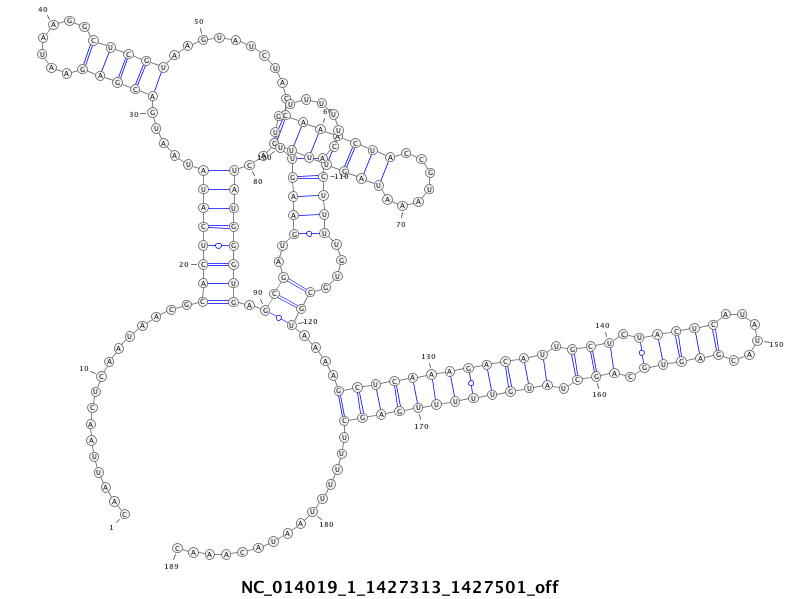
\includegraphics[width=.45\linewidth]{Figures/NC_014019_1_1427313_1427501_off.png}
    \hfill
    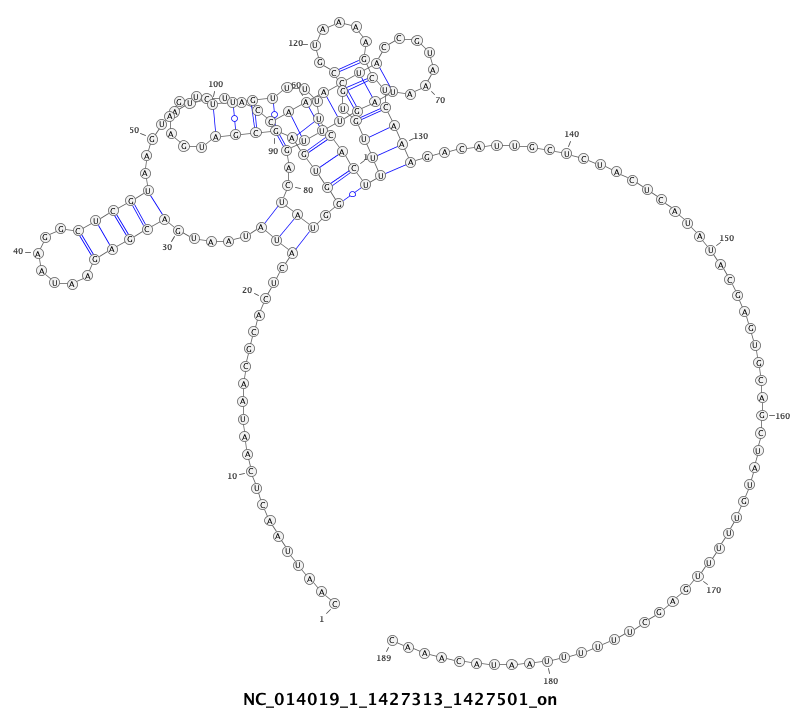
\includegraphics[width=.45\linewidth]{Figures/NC_014019_1_1427313_1427501_on.png}
    \caption{{\em Left:} the computationally predicted gene-off conformation of sequence NC\_014019.1 1427313-1427501, using \ms{RNAfold} from the ViennaRNA 2.1.8 suite, with dangles disabled and the Turner 1999 energies. This sequence is located upstream of the xpt gene in Bacillus megaterium QM B1551. {\em Right:} the gene-on conformation.}
  \label{fig:example_ss}
\end{figure}

\subsection{Fine-Grained Filtering} \label{sub:fine}

Until now, we have described our approach for generating the 503 guanine riboswitch candidates in RefSeq, alongside their gene-on and off structures. Unfortunately the experimental validation of all 503 candidates is not tractable, so it was necessary to reduce this collection again to a more manageable size, while only keeping the most promising candidates.

\subsubsection{Using \foldalign to Rank Candidates} \label{ssub:foldalign}
 
%\input{Chapters/Chapter3}
%\input{Chapters/Chapter4} 
%\input{Chapters/Chapter5} 
%\input{Chapters/Chapter6} 
%\input{Chapters/Chapter7} 

%----------------------------------------------------------------------------------------
%	THESIS CONTENT - APPENDICES
%----------------------------------------------------------------------------------------

\addtocontents{toc}{\vspace{2em}} % Add a gap in the Contents, for aesthetics

\appendix % Cue to tell LaTeX that the following 'chapters' are Appendices

% Include the appendices of the thesis as separate files from the Appendices folder
% Uncomment the lines as you write the Appendices

% Appendix A

\chapter{Appendix Title Here} % Main appendix title

\label{AppendixA} % For referencing this appendix elsewhere, use \ref{AppendixA}

\lhead{Appendix A. \emph{Appendix Title Here}} % This is for the header on each page - perhaps a shortened title

Write your Appendix content here.
%\input{Appendices/AppendixB}
%\input{Appendices/AppendixC}

\addtocontents{toc}{\vspace{2em}} % Add a gap in the Contents, for aesthetics

\backmatter

%----------------------------------------------------------------------------------------
%	BIBLIOGRAPHY
%----------------------------------------------------------------------------------------

\label{Bibliography}

\lhead{\emph{Bibliography}} % Change the page header to say "Bibliography"

\bibliographystyle{unsrtnat} % Use the "unsrtnat" BibTeX style for formatting the Bibliography

\bibliography{Bibliography} % The references (bibliography) information are stored in the file named "Bibliography.bib"

\end{document}  